\documentclass{amsart} 
\usepackage{amsmath}
\DeclareMathOperator*{\argmax}{arg\,max}
\DeclareMathOperator*{\argmin}{arg\,min}
\usepackage{graphicx}
\graphicspath{{./}}
\usepackage[fontsize=14pt]{scrextend}
\usepackage{hyperref}
\usepackage{csvsimple}
\usepackage{longtable}
\usepackage{epigraph}
\title{Order in Human Nature}
\author{Zulfikar Moinuddin Ahmed}
\date{\today}
\begin{document}
\maketitle

\section{Classical Orientation: Fate and Eternal Recurrence}

My point of view about the universe in which we live and all things in it, all things that have objective existence and the laws that govern this Existence is quite different from most empiricists of this age.  There is a history for this too, for when I was young, I was much more enthusiastic about philosophy, literature, and mathematics; and I was friends with many much more directly interested in natural sciences but I was not in their camp.  I was deeply internal, and my intellectual gifts were more in mathematics and literature.  In my four years at Princeton, despite many friends quite enthusiastic about physics, and despite meeting many friends in my mathematics courses, I did not take a single physics course.  My convictions had grown over time against expansionary cosmology, of all people, from Percy Bysshe Shelley, and I was quite excited in around 2012 in San Francisco when I lived in a hovel -- a rented room of a Hotel--as an apartment on 22nd and Valencia or Mission. I was euphoric because my guess that the redshift slope was completely explainable by the curvature of a four-sphere and is pure geometric error was looking quite good already.  I had read articles about 'accelerating expansion' but I dismissed them as erroneous and continued.  I have shown that the Law of Fate is one, S4 Electromagnetism, a classical deterministic law behind all things of Heaven and Earth.

\section{Six million years of human evolution from chimpanzee-cousins has recurred infinitely many times on Earth}

Eternal Recurrence is proven with Four-Sphere Theory, and therefore, we can conclude quite strongly that the evolution of Man occurred on Earth an infinitely many times in the past.  The time spans between recurrence are vast, in the order of $10^{21} years$, and thus it may not seem relevant to our understanding of human evolution, but it is in various ways that I will come to another day.  

\section{Moral Laws of Human Race}

I discovered that there is strong universality for moral opinion across the world.  Good and Evil are interpolated by exponential law favouring Good.

\section{Case of Opinions on Stealing}

I am not going to worry about the gap between opinions about stealing and actual occurrences of stealing.  I am using World Values Survey.  

\section{Distribution of Exponential Lambda Parameters for Stealing}

For Q179 "Stealing is justified" from never to always in 10 steps, we fit exponential models for 49 countries.

\subsection{Tightness of the distribution}

The mean lambda is $\bar{\lambda} = -0.49$ and the standard deviation is $\sigma(\lambda) = 0.1825$.  I will show a good Generalised Hyperbolic Distribution fit to the distribution below.  But we note that the dispersion is quite tight for the fitted exponential parameter model $\lambda$ across 49 countries.  {\em This tightness} of the dispersion is the most important scientific discovery here for stealing across the globe, for this is what indicates the Human Nature regularity of the actually held moral value regarding stealing across the globe.  And because this is so small, we have evidence then that the regularity has primarily evolutionary explanations, that our moral values are universally regular and roughly independent of ethnicity, religion, nation,culture.

\section{Histogram and GHD Fit}

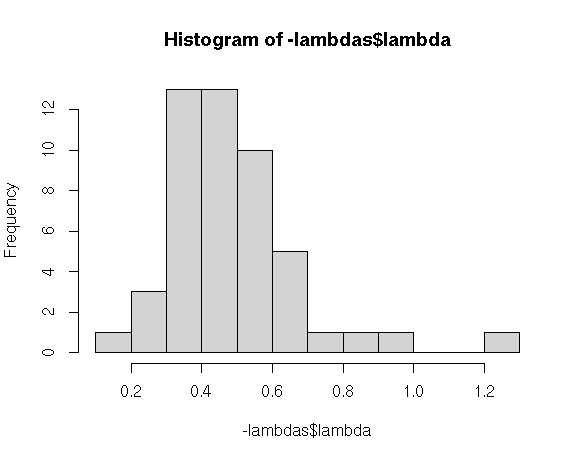
\includegraphics[scale=1.0]{stld.png}

\begin{verbatim}
> summary(fit.steal)
Asymmetric Generalized Hyperbolic Distribution:

Parameters:
    lambda  alpha.bar         mu      sigma      gamma 
-1.9407775  0.7321604  0.3897397  0.1496352  0.1007499 

Call:
fit.ghypuv(data = -lambdas$lambda)

Optimization information:
log-Likelihood:                21.2762 
AIC:                           -32.5524 
Fitted parameters:             lambda, alpha.bar, mu, sigma, gamma;  (Number: 5)
Number of iterations:          424 
Converged:                     TRUE 
\end{verbatim}

\section{Data}

% latex table generated in R 4.0.3 by xtable 1.8-4 package
% Wed Apr 21 03:41:27 2021
\begin{longtable}{rrr}
  \hline
 & B\_COUNTRY & lambda \\ 
  \hline
1 & 20 & -0.6989 \\ 
  2 & 32 & -0.4599 \\ 
  3 & 36 & -0.4950 \\ 
  4 & 50 & -0.9361 \\ 
  5 & 68 & -0.4828 \\ 
  6 & 76 & -0.3450 \\ 
  7 & 152 & -0.3837 \\ 
  8 & 156 & -0.5327 \\ 
  9 & 170 & -0.3903 \\ 
  10 & 196 & -0.4712 \\ 
  11 & 276 & -0.8512 \\ 
  12 & 218 & -0.3500 \\ 
  13 & 818 & -1.2102 \\ 
  14 & 231 & -0.3797 \\ 
  15 & 300 & -0.6223 \\ 
  16 & 320 & -0.3188 \\ 
  17 & 344 & -0.5017 \\ 
  18 & 360 & -0.5128 \\ 
  19 & 364 & -0.4998 \\ 
  20 & 368 & -0.4436 \\ 
  21 & 400 & -0.4897 \\ 
  22 & 392 & -0.6140 \\ 
  23 & 398 & -0.3701 \\ 
  24 & 417 & -0.3402 \\ 
  25 & 410 & -0.5730 \\ 
  26 & 422 & -0.5346 \\ 
  27 & 446 & -0.5377 \\ 
  28 & 484 & -0.3072 \\ 
  29 & 104 & -0.7828 \\ 
  30 & 458 & -0.2545 \\ 
  31 & 566 & -0.4897 \\ 
  32 & 558 & -0.3416 \\ 
  33 & 554 & -0.5066 \\ 
  34 & 586 & -0.3666 \\ 
  35 & 604 & -0.4735 \\ 
  36 & 608 & -0.1853 \\ 
  37 & 630 & -0.3674 \\ 
  38 & 642 & -0.4342 \\ 
  39 & 643 & -0.3964 \\ 
  40 & 688 & -0.2140 \\ 
  41 & 764 & -0.5826 \\ 
  42 & 762 & -0.6452 \\ 
  43 & 788 & -0.5453 \\ 
  44 & 792 & -0.4669 \\ 
  45 & 158 & -0.6317 \\ 
  46 & 804 & -0.5153 \\ 
  47 & 840 & -0.4587 \\ 
  48 & 704 & -0.4533 \\ 
  49 & 716 & -0.2676 \\ 
   \hline
\hline
\end{longtable}

\section{Implications}
Jurisprudence on Earth can improve vastly if laws focused on treating the outliers only.  The most important factors are that the mothers have time to form secure attachments with children, and fathers are present and can guide adolescents.  After this, coercive exesses is a burden on the populations and these $\lambda$ for stealing cannot be affected strongly by use of coercive techniques.  Prudent strategies to understand human nature in quantitative terms will reduce costs of law enforcement, and our results are totally independent on wealth, ethnicity, religion, culture.

\end{document}
